\section{Introduction}
Nowadays, Internet-of-Things (IoT) technologies have been used in many different fields (e.g., smart home and smart
campus) for providing convenience and efficiency to users. Similarly, this paper proposes an automatic attendance system
different from existing attendance systems. The existing attendance systems are usually operated by a manual methodor
elec-trical system by identifying a student identification (ID) card or using an attendance application. There are some
problems in these systems.
For example, there is lecture time loss because of checking attendance by a manual method.
Also, if students use an electrical attendance system, they always need to carry their student ID card or smartphone with
an attendance application. A proxy at- tendance (i.e., attendance of somebody else for the sake of a person) can be done
by an unconscionable person. This weak point of the existing attendance systems should be prevented
Maintaining the attendance is very important in all the institutes for checking the performance of employees. Every
institute has its own method in this regard. Some are taking attendance manually using the old paper or file based approach
and some have adopted methods of automatic attendance using some bio-metric techniques.
But in these methods employees have to wait for long time in making a queue at time they enter the office. Many biometric systems are available but the key au-thenti cations are same is all the techniques.
Our system uses the face recognition approach for the automatic attendance of employees in the office room environment
without employees’ intervention Face recognition consists of two steps, in first step faces are detected in the image and
then these detected faces are compared with the database for verification. A num- ber of methods have been proposed for
face detection i.e. Ada Boost algorithm, the Float Boost algorithm, the S-Ada Boost algorithm Support Vector Machines
(SVM), and the Bayes classifier
\\
A facial recognition system[1] is a technology potentially capable of matching a human face from a digital image or a video frame against a database of faces. Such a system is typically employed to authenticate users through ID verification services, and works by pinpointing and measuring facial features from a given image.[2]

Development began on similar systems in the 1960s, beginning as a form of computer application. Since their inception, facial recognition systems have seen wider uses in recent times on smartphones and in other forms of technology, such as robotics. Because computerized facial recognition involves the measurement of a human's physiological characteristics, facial recognition systems are categorized as biometrics. Although the accuracy of facial recognition systems as a biometric technology is lower than iris recognition, fingerprint image acquisition, palm recognition or voice recognition, it is widely adopted due to its contactless process.[3] Facial recognition systems have been deployed in advanced human–computer interaction, video surveillance, law enforcement, passenger screening, decisions on employment and housing and automatic indexing of images.[4][5]

Facial recognition systems are employed throughout the world today by governments and private companies.[6] Their effectiveness varies, and some systems have previously been scrapped because of their ineffectiveness. The use of facial recognition systems has also raised controversy, with claims that the systems violate citizens' privacy, commonly make incorrect identifications, encourage gender norms[7][8] and racial profiling,[9] and do not protect important biometric data. The appearance of synthetic media such as deepfakes has also raised concerns about its security.[10] These claims have led to the ban of facial recognition systems in several cities in the United States.[11] Growing societal concerns led social networking company Meta Platforms to shut down its Facebook facial recognition system in 2021, deleting the face scan data of more than one billion users.[12][13] The change represented one of the largest shifts in facial recognition usage in the technology's history.
\newpage
\section{Project Objective: }

Attendance is prime important for both the teacher and student of an educational organization. So it is very important to keep record of the attendance. The problem arises when we think about the traditional process of taking attendance in class room. 
Calling name or roll number of the student for attendance is not only a problem of time consumption but also it needs energy. So an automatic attendance system can solve all above problems. 
There are some automatic attendances making system which are currently used by much institution. One of such system is biometric technique and RFID system. Although it is automatic and a step ahead of traditional method it fails to meet the time constraint. The student has to wait in queue for giving attendance, which is time taking. 
This project introduces an involuntary attendance marking system, devoid of any kind of interference with the normal teaching procedure. The system can be also implemented during exam sessions or in other teaching activities where attendance is highly essential. This system eliminates classical student identification such as calling name of the student, or checking respective identification cards of the student, which can not only interfere with the ongoing teaching process, but also can be stressful for students during examination sessions. In addition, the students have to register in the database to be recognized. The enrolment can be done on the spot through the userfriendly interface. 
\newpage
\section{Problem Statement: }
Traditional student attendance marking technique is often facing a lot of trouble. The face recognition student attendance system emphasizes its simplicity by eliminating classical student attendance marking technique such as calling student names or checking respective identification cards. There are not only disturbing the teaching process but also causes distraction for students during exam sessions. Apart from calling names, attendance sheet is passed around the classroom during the lecture sessions. The lecture class especially the class with a large number of students might find it difficult to have the attendance sheet being passed around the class. Thus, face recognition attendance system is proposed in order to replace the manual signing of the presence of students which are burdensome and causes students get distracted in order to sign for their attendance. Furthermore, the face recognition based automated student attendance system able to overcome the problem of fraudulent approach and lecturers does not have to count the number of students several times to ensure the presence of the students. 
 
 The paper proposed by Zhao, W et al. (2003) has listed the difficulties of facial identification. One of the difficulties of facial identification is the identification between known and unknown images. In addition, paper proposed by Pooja G.R et al. (2010) found out that the training process for face recognition student attendance system is slow and time-consuming. In addition, the paper proposed by Priyanka Wagh et al. (2015) mentioned that different lighting and head poses are often the problems that could degrade the performance of face recognition based student attendance system. 
 Hence, there is a need to develop a real time operating student attendance system which means the identification process must be done within defined time constraints to prevent omission. The extracted features from facial images which represent the identity of the students have to be consistent towards a change in background, illumination, pose and expression. High accuracy and fast computation time will be the evaluation points of the performance. 
 \newpage
\section{Scope of the project: }
We are setting up to design a system comprising of two modules. The first module (face detector) is a mobile component, which is basically a camera application that captures student faces and stores them in a file using computer vision face detection algorithms and face extraction techniques. The second module is a desktop application that does face recognition of the captured images (faces) in the file, marks the students register and then stores the results in a database for future analysis. 
\newpage
\section{Background :}
The human face is a unique representation of individual identity. Thus, face recognition is defined as a biometric method in which identification of an individual is performed by comparing real-time capture image with stored images in the database of that person (Margaret Rouse, 2012). 
Nowadays, face recognition system is prevalent due to its simplicity and awesome performance. For instance, airport protection systems and FBI use face recognition for criminal investigations by tracking suspects, missing children and drug activities (Robert Silk, 2017). Apart from that, Facebook which is a popular social networking website implement face recognition to allow the users to tag their friends in the photo for entertainment purposes (Sidney Fussell, 2018). Furthermore, Intel Company allows the users to use face recognition to get access to their online account (Reichert, C., 2017). Apple allows the users to unlock their mobile phone, iPhone X by using face recognition (deAgonia, M., 2017). 
The work on face recognition began in 1960. Woody Bledsoe, Helen Chan Wolf and Charles Bisson had introduced a system which required the administrator to locate eyes, ears, nose and mouth from images. The distance and ratios between the located features and the common reference points are then calculated and compared. The studies are further enhanced by Goldstein, Harmon, and Lesk in 1970 by using other features such as hair colour and lip thickness to automate the recognition. In 1988, Kirby and Sirovich first suggested principle component analysis (PCA) to solve face recognition problem. Many studies on face recognition were then conducted continuously until today (Ashley DuVal, 2012). 


\newpage
\section{COMPONENT DESCRIPTION
}
\section{Landing Page :}
This is basically the Home page of our Project. After opening the system this is the first page user will see. In this the
user can able to Register, By adding First Name, Last Name, Address, Status and mobile number. Once user submitted
his data, then we have to create our face data and train it. Then user can mark his attendance by clicking on the button
called face attendance.
And once attendance has been marked successfully, user’s care taker got notification on email.
\newpage
\section{Scope of the project: }
We are setting up to design a system comprising of two modules. The first module (face detector) is a mobile component, which is basically a camera application that captures student faces and stores them in a file using computer vision face detection algorithms and face extraction techniques. The second module is a desktop application that does face recognition of the captured images (faces) in the file, marks the students register and then stores the results in a database for future analysis. 
\newpage

\section{Register:}

This page provides the facility for the user to register and create a new account for only one time. This system provides
options of status so that user can register as an instructor or as a student. For registering, any user requires to fill-up the
following form box of First Name, Last Name, Address, Status and Mobile Number.
There are validations added for this form such as the Display, Soo user can Re-check he is registered successfully or not.
Also he can take look on the personal information has been submitted
         


\newpage
\section{Create Face Data :}
This page basically helps to capture or create the image data set. At a time, it takes 24 images of every user by different
angels. Soo user don’t need to wait or pass through front of camera everytime .
Also We can add User Id for every user at the time of creating face data.
\newpage
\section{Train Face Data :}
This Page Train the face data, that we created already. Every Time when we added new user data, This programming
page train, identify, manage all stored data. It can neglect the unwanted things from images , and crop, reduce the size of
images and soo on
\newpage
\section{Application}
\section{Social media}
Founded in 2013, Looksery went on to raise money for its face modification app on Kickstarter. After successful crowdfunding, Looksery launched in October 2014. The application allows video chat with others through a special filter for faces that modifies the look of users. Image augmenting applications already on the market, such as Facetune and Perfect365, were limited to static images, whereas Looksery allowed augmented reality to live videos. In late 2015 SnapChat purchased Looksery, which would then become its landmark lenses function.[55] Snapchat filter applications use face detection technology and on the basis of the facial features identified in an image a 3D mesh mask is layered over the face.[56]

DeepFace is a deep learning facial recognition system created by a research group at Facebook. It identifies human faces in digital images. It employs a nine-layer neural net with over 120 million connection weights, and was trained on four million images uploaded by Facebook users.[57][58] The system is said to be 97% accurate, compared to 85% for the FBI's Next Generation Identification system.
\newpage
\section{ID verification}
The emerging use of facial recognition is in the use of ID verification services. Many companies and others are working in the market now to provide these services to banks, ICOs, and other e-businesses.[63] Face recognition has been leveraged as a form of biometric authentication for various computing platforms and devices;[36] Android 4.0 "Ice Cream Sandwich" added facial recognition using a smartphone's front camera as a means of unlocking devices,[64][65] while Microsoft introduced face recognition login to its Xbox 360 video game console through its Kinect accessory,[66] as well as Windows 10 via its "Windows Hello" platform (which requires an infrared-illuminated camera).[67] In 2017, Apple's iPhone X smartphone introduced facial recognition to the product line with its "Face ID" platform, which uses an infrared illumination system
\newpage
\section{Face ID}
Apple introduced Face ID on the flagship iPhone X as a biometric authentication successor to the Touch ID, a fingerprint based system. Face ID has a facial recognition sensor that consists of two parts: a "Romeo" module that projects more than 30,000 infrared dots onto the user's face, and a "Juliet" module that reads the pattern.[69] The pattern is sent to a local "Secure Enclave" in the device's central processing unit (CPU) to confirm a match with the phone owner's face.[70]

The facial pattern is not accessible by Apple. The system will not work with eyes closed, in an effort to prevent unauthorized access.[70] The technology learns from changes in a user's appearance, and therefore works with hats, scarves, glasses, and many sunglasses, beard and makeup.[71] It also works in the dark. This is done by using a "Flood Illuminator", which is a dedicated infrared flash that throws out invisible infrared light onto the user's face to properly read the 30,000 facial points.
\newpage
\section{Healthcare}
Facial recognition algorithms can help in diagnosing some diseases using specific features on the nose, cheeks and other part of the human face.[73] Relying on developed data sets, machine learning has been used to identify genetic abnormalities just based on facial dimensions.[74] FRT has also been used to verify patients before surgery procedures.

In March, 2022 according to a publication by Forbes, FDNA, an AI development company claimed that in the space of 10 years, they have worked with geneticists to develop a database of about 5,000 diseases and 1500 of them can be detected with facial recognition algorithms
\newpage
\section{ALGORITHM :}
{Haar Cascade Algorithm :} Haar Cascade is a feature-based object detection algorithm to detect objects from images. A cascade function is trained
on lots of positive and negative images for detection. The algorithm does not require extensive computation and can run
in real-time
In this article, we are going to see how to detect faces using a cascade classifier in OpenCV Python. Face detection has
much significance in different fields of today’s world. It is a significant step in several applications, face recognition
(also used as biometrics), photography (for auto-focus on the face), face analysis (age, gender, emotion recognition),
video surveillance, etc
One of the popular algorithms for facial detection is “haarcascade”. It is computationally less expensive, a fast
algorithm, and gives high accuracy.

\section{Haar-feature selection:}A Haar-like feature consists of dark regions and light regions. It produces a single value by taking the difference of
the sum of the intensities of the dark regions and the sum of the intensities of light regions. It is done to extract
useful elements necessary for identifying an object. The features proposed 
\newpage
\section{Deployment in security services}
\section{India}
Even though facial recognition technology (FRT) is not fully accurate,[112] it is being increasingly deployed for identification purposes by the police in India. FRT systems generate a probability match score, or a confidence score between the suspect who is to be identified and the database of identified criminals that is available with the police. The National Automated Facial Recognition System (AFRS)[113] is already being developed by the National Crime Records Bureau (NCRB), a body constituted under the Ministry of Home Affairs. The project seeks to develop and deploy a national database of photographs which would comport with a facial recognition technology system by the central and state security agencies. The Internet Freedom Foundation has flagged concerns regarding the project.[114] The NGO has highlighted that the accuracy of FRT systems are "routinely exaggerated and the real numbers leave much to be desired.[114] The implementation of such faulty FRT systems would lead to high rates of false positives and false negatives in this recognition process." 

Under the Supreme Court of India's decision in Justice K.S. Puttaswamy vs Union of India (22017 10 SCC 1), any justifiable intrusion by the State into people's right to privacy, which is protected as a fundamental right under Article 21 of the Constitution, must confirm to certain thresholds, namely: legality, necessity, proportionality and procedural safeguards.[115] As per the Internet Freedom Foundation, the National Automated Facial Recognition System (AFRS) proposal fails to meet any of these thresholds, citing "absence of legality," "manifest arbitrariness," and "absence of safeguards and accountability."[116]

While the national level AFRS project is still in the works, police departments in various states in India are already deploying facial recognition technology systems, such as: TSCOP + CCTNS in Telangana,[117] Punjab Artificial Intelligence System (PAIS) in Punjab,[118] Trinetra in Uttar Pradesh,[119] Police Artificial Intelligence System in Uttarakhand,[120] AFRS in Delhi, Automated Multimodal Biometric Identification System (AMBIS) in Maharashtra, FaceTagr in Tamil Nadu. The Crime and Criminal Tracking Network and Systems (CCTNS), which is a Mission Mode Project under the National e-Governance Plan (NeGP),[121] is viewed as a system which would connect police stations across India, and help them "talk"[122] to each other. The project's objective is to digitize all FIR-related information, including FIRs registered, as well as cases investigated, charge sheets filed, and suspects and wanted persons in all police stations. This shall constitute a national database of crime and criminals in India. CCTNS is being implemented without a data protection law in place. CCTNS is proposed to be integrated with the AFRS, a repository of all crime and criminal related facial data which can be deployed to purportedly identify or verify a person from a variety of inputs ranging from images to videos.[123] This has raised privacy concerns from civil society organizations and privacy experts. Both the projects have been censured as instruments of "mass surveillance" at the hands of the state.[124] In Rajasthan, 'RajCop,' a police app has been recently integrated with a facial recognition module which can match the face of a suspect against a database of known persons in real-time. Rajasthan police is in currently working to widen the ambit of this module by making it mandatory to upload photographs of all arrested persons in CCTNS database, which will "help develop a rich database of known offenders."[125]

Helmets fixed with camera have been designed and being used by Rajasthan police in law and order situations to capture police action and activities of "the miscreants, which can later serve as evidence during the investigation of such cases."[125] PAIS (Punjab Artificial Intelligence System), App employs deep learning, machine learning, and face recognition for the identification of criminals to assist police personnel.[125] The state of Telangana has installed 8 lakh CCTV cameras,[125] with its capital city Hyderabad slowly turning into a surveillance capital.[126]

A false positive happens when facial recognition technology misidentifies a person to be someone they are not, that is, it yields an incorrect positive result. They often results in discrimination and strengthening of existing biases. For example, in 2018, Delhi Police reported that its FRT system had an accuracy rate of 2%, which sank to 1% in 2019. The FRT system even failed to distinguish accurately between different sexes.[127]

The government of Delhi in collaboration with Indian Space Research Organisation (ISRO) is developing a new technology called Crime Mapping Analytics and Predictive System (CMAPS). The project aims to deploy space technology for "controlling crime and maintaining law and order."[125] The system will be connected to a database containing data of criminals.[125] The technology is envisaged to be deployed to collect real-time data at the crime scene.[125]

In a reply dated November 25, 2020 to a Right to Information request filed by the Internet Freedom Foundation seeking information about the facial recognition system being used by the Delhi Police (with reference number DEPOL/R/E/20/07128),[128] the Office of the Deputy Commissioner of Police cum Public Information Officer: Crime stated that they cannot provide the information under section 8(d) of the Right to Information Act, 2005.[129] A Right to Information (RTI) request dated July 30, 2020 was filed with the Office of the Commissioner, Kolkata Police, seeking information about the facial recognition technology that the department was using.[130] The information sought was denied[131] stating that the department was exempted from disclosure under section 24(4) of the RTI Act.
\newpage
\section{Advantages and disadvantages}
\section{Compared to other biometric systems}
In 2006, the performance of the latest face recognition algorithms was evaluated in the Face Recognition Grand Challenge (FRGC). High-resolution face images, 3-D face scans, and iris images were used in the tests. The results indicated that the new algorithms are 10 times more accurate than the face recognition algorithms of 2002 and 100 times more accurate than those of 1995. Some of the algorithms were able to outperform human participants in recognizing faces and could uniquely identify identical twins.[44][158]

One key advantage of a facial recognition system that it is able to perform mass identification as it does not require the cooperation of the test subject to work. Properly designed systems installed in airports, multiplexes, and other public places can identify individuals among the crowd, without passers-by even being aware of the system.[159] However, as compared to other biometric techniques, face recognition may not be most reliable and efficient. Quality measures are very important in facial recognition systems as large degrees of variations are possible in face images. Factors such as illumination, expression, pose and noise during face capture can affect the performance of facial recognition systems.[159] Among all biometric systems, facial recognition has the highest false acceptance and rejection rates,[159] thus questions have been raised on the effectiveness of or bias of face recognition software in cases of railway and airport security, law enforcement and housing and employment decisions
\newpage
\section{Weaknesses}
Ralph Gross, a researcher at the Carnegie Mellon Robotics Institute in 2008, describes one obstacle related to the viewing angle of the face: "Face recognition has been getting pretty good at full frontal faces and 20 degrees off, but as soon as you go towards profile, there've been problems."[44] Besides the pose variations, low-resolution face images are also very hard to recognize. This is one of the main obstacles of face recognition in surveillance systems.[161] It has also been suggested that camera settings can favour sharper imagery of white skin than of other skin tones.[5]

Face recognition is less effective if facial expressions vary. A big smile can render the system less effective. For instance: Canada, in 2009, allowed only neutral facial expressions in passport photos.[162]

There is also inconstancy in the datasets used by researchers. Researchers may use anywhere from several subjects to scores of subjects and a few hundred images to thousands of images. Data sets may be diverse and inclusive or mainly contain images of white males. It is important for researchers to make available the datasets they used to each other, or have at least a standard or representative dataset.[163]

Although high degrees of accuracy have been claimed for some facial recognition systems, these outcomes are not universal. The consistently worst accuracy rate is for those who are 18 to 30 years old, Black and female.[5]

Facial recognition systems have been criticized for upholding and judging based on assumptions about people of colour [164] and also on a binary gender assumption.[165][166][167][168][169][170][171][172][173] When classifying the faces of cisgender individuals into male or female, these systems are often fairly accurate,[165] however were typically confused or unable to determine the gender identity of transgender and non-binary people.[165] Gender norms are being upheld by these systems, so much so that even when shown a photo of a cisgender male with long hair, algorithms was split between following the gender norm of males having short hair, and the masculine facial features and became confused.[165][173] This accidental misgendering of people can be very harmful for those who do not identify with their sex assigned at birth, by disregarding and invalidating their gender identity. This is also harmful for people who do not ascribe to traditional gender norms, because it invalidates their gender expression, regardless of their gender identity.
\newpage
\section{Ineffectiveness}
Critics of the technology complain that the London Borough of Newham scheme has, as of 2004, never recognized a single criminal, despite several criminals in the system's database living in the Borough and the system has been running for several years. "Not once, as far as the police know, has Newham's automatic face recognition system spotted a live target."[148][174] This information seems to conflict with claims that the system was credited with a 34% reduction in crime (hence why it was rolled out to Birmingham also).[175]

An experiment in 2002 by the local police department in Tampa, Florida, had similarly disappointing results.[148] A system at Boston's Logan Airport was shut down in 2003 after failing to make any matches during a two-year test period.[176]

In 2014, Facebook stated that in a standardized two-option facial recognition test, its online system scored 97.25% accuracy, compared to the human benchmark of 97.5%.[177]

Systems are often advertised as having accuracy near 100%; this is misleading as the outcomes are not universal[5] The studies often use samples that are smaller and less diverse than would be necessary for large scale applications. Because facial recognition is not completely accurate, it creates a list of potential matches. A human operator must then look through these potential matches and studies show the operators pick the correct match out of the list only about half the time. This causes the issue of targeting the wrong suspect


\newpage
\section{Creation of Integral Images:}
A given pixel in the integral image is the sum of all the pixels on the left and all the pixels above it. Since the
process of extracting Haar-like features involves calculating the difference of dark and light rectangular regions, the
introduction of Integral Images reduces the time needed to complete this task significantly

\section{AdaBoost Training:}This algorithm selects the best features from all features. It combines multiple “weak classifiers” (best features) into
one “strong classifier”. The generated “strong classifier” is basically the linear combination of all “weak classifiers”.
\section{Controversies}
\section{Privacy violations}
Civil rights organizations and privacy campaigners such as the Electronic Frontier Foundation, Big Brother Watch and the ACLU express concern that privacy is being compromised by the use of surveillance technologies.[179][84][180] Face recognition can be used not just to identify an individual, but also to unearth other personal data associated with an individual – such as other photos featuring the individual, blog posts, social media profiles, Internet behavior, and travel patterns.[181] Concerns have been raised over who would have access to the knowledge of one's whereabouts and people with them at any given time.[182] Moreover, individuals have limited ability to avoid or thwart face recognition tracking unless they hide their faces. This fundamentally changes the dynamic of day-to-day privacy by enabling any marketer, government agency, or random stranger to secretly collect the identities and associated personal information of any individual captured by the face recognition system.[181] Consumers may not understand or be aware of what their data is being used for, which denies them the ability to consent to how their personal information gets shared.[182]

In July 2015, the United States Government Accountability Office conducted a Report to the Ranking Member, Subcommittee on Privacy, Technology and the Law, Committee on the Judiciary, U.S. Senate. The report discussed facial recognition technology's commercial uses, privacy issues, and the applicable federal law. It states that previously, issues concerning facial recognition technology were discussed and represent the need for updating the privacy laws of the United States so that federal law continually matches the impact of advanced technologies. The report noted that some industry, government, and private organizations were in the process of developing, or have developed, "voluntary privacy guidelines". These guidelines varied between the stakeholders, but their overall aim was to gain consent and inform citizens of the intended use of facial recognition technology. According to the report the voluntary privacy guidelines helped to counteract the privacy concerns that arise when citizens are unaware of how their personal data gets put to use.[182]

In 2016, Russian company NtechLab caused a privacy scandal in the international media when it launched the FindFace face recognition system with the promise that Russian users could take photos of strangers in the street and link them to a social media profile on the social media platform Vkontakte (VT).[183] In December 2017, Facebook rolled out a new feature that notifies a user when someone uploads a photo that includes what Facebook thinks is their face, even if they are not tagged. Facebook has attempted to frame the new functionality in a positive light, amidst prior backlashes.[184] Facebook's head of privacy, Rob Sherman, addressed this new feature as one that gives people more control over their photos online. "We've thought about this as a really empowering feature," he says. "There may be photos that exist that you don't know about."[185] Facebook's DeepFace has become the subject of several class action lawsuits under the Biometric Information Privacy Act, with claims alleging that Facebook is collecting and storing face recognition data of its users without obtaining informed consent, in direct violation of the 2008 Biometric Information Privacy Act (BIPA).[186] The most recent case was dismissed in January 2016 because the court lacked jurisdiction.[187] In the US, surveillance companies such as Clearview AI are relying on the First Amendment to the United States Constitution to data scrape user accounts on social media platforms for data that can be used in the development of facial recognition systems.[188]

In 2019, the Financial Times first reported that facial recognition software was in use in the King's Cross area of London.[189] The development around London's King's Cross mainline station includes shops, offices, Google's UK HQ and part of St Martin's College. According to the UK Information Commissioner's Office: "Scanning people's faces as they lawfully go about their daily lives, in order to identify them, is a potential threat to privacy that should concern us all."[190][191] The UK Information Commissioner Elizabeth Denham launched an investigation into the use of the King's Cross facial recognition system, operated by the company Argent. In September 2019 it was announced by Argent that facial recognition software would no longer be used at King's Cross. Argent claimed that the software had been deployed between May 2016 and March 2018 on two cameras covering a pedestrian street running through the centre of the development.[192] In October 2019, a report by the deputy London mayor Sophie Linden revealed that in a secret deal the Metropolitan Police had passed photos of seven people to Argent for use in their King's cross facial recognition system.[193]

Automated Facial Recognition was trialled by the South Wales Police on multiple occasions between 2017 and 2019. The use of the technology was challenged in court by a private individual, Edward Bridges, with support from the charity Liberty (case known as R (Bridges) v Chief Constable South Wales Police). The case was heard in the Court of Appeal and a judgement was given in August 2020.[194] The case argued that the use of Facial Recognition was a privacy violation on the basis that there was insufficient legal framework or proportionality in the use of Facial Recognition and that its use was in violation of the Data Protection Acts 1998 and 2018. The case was decided in favour of Bridges and did not award damages. The case was settled via a declaration of wrongdoing.[194] In response to the case, the British Government has repeatedly attempted to pass a Bill regulating the use of Facial Recognition in public spaces. The proposed Bills have attempted to appoint a Commissioner with the ability to regulate Facial Recognition use by Government Services in a similar manner to the Commissioner for CCTV. Such a Bill has yet to come into force [correct as of September 2021].[118]

In January 2023, New York Attorney General Letitia James asked for more information on the use of facial recognition technology from Madison Square Garden Entertainment following reports that the firm used it to block lawyers involved in litigation against the company from entering Madison Square Garden. She noted such a move would could go against federal, state, and local human rights laws
\newpage
\section{Imperfect technology in law enforcement}
As of 2018, it is still contested as to whether or not facial recognition technology works less accurately on people of color.[196] One study by Joy Buolamwini (MIT Media Lab) and Timnit Gebru (Microsoft Research) found that the error rate for gender recognition for women of color within three commercial facial recognition systems ranged from 23.8% to 36%, whereas for lighter-skinned men it was between 0.0 and 1.6%. Overall accuracy rates for identifying men (91.9%) were higher than for women (79.4%), and none of the systems accommodated a non-binary understanding of gender.[197] It also showed that the datasets used to train commercial facial recognition models were unrepresentative of the broader population and skewed toward lighter-skinned males. However, another study showed that several commercial facial recognition software sold to law enforcement offices around the country had a lower false non-match rate for black people than for white people.[198]

Experts fear that face recognition systems may actually be hurting citizens the police claims they are trying to protect.[199] It is considered an imperfect biometric, and in a study conducted by Georgetown University researcher Clare Garvie, she concluded that "there's no consensus in the scientific community that it provides a positive identification of somebody."[200] It is believed that with such large margins of error in this technology, both legal advocates and facial recognition software companies say that the technology should only supply a portion of the case – no evidence that can lead to an arrest of an individual.[200] The lack of regulations holding facial recognition technology companies to requirements of racially biased testing can be a significant flaw in the adoption of use in law enforcement. CyberExtruder, a company that markets itself to law enforcement said that they had not performed testing or research on bias in their software. CyberExtruder did note that some skin colors are more difficult for the software to recognize with current limitations of the technology. "Just as individuals with very dark skin are hard to identify with high significance via facial recognition, individuals with very pale skin are the same," said Blake Senftner, a senior software engineer at CyberExtruder.[200]

The United States' National Institute of Standards and Technology (NIST) carried out extensive testing of FRT system 1:1 verification[201] and 1:many identification.[201] It also tested for the differing accuracy of FRT across different demographic groups. The independent study concluded at present, no FRT system has 100% accuracy.

\newpage
\section{Cascade Classifier:}
It is a method for combining increasingly more complex classifiers like AdaBoost in a cascade which allows
negative input (non-face) to be quickly discarded while spending more computation on promising or positive facelike regions. It significantly reduces the computation time and makes the process more efficient.
OpenCV comes with lots of pre-trained classifiers. Those XML files can be loaded by cascade Classifier method of



\section{Stepwise Implementation:
}
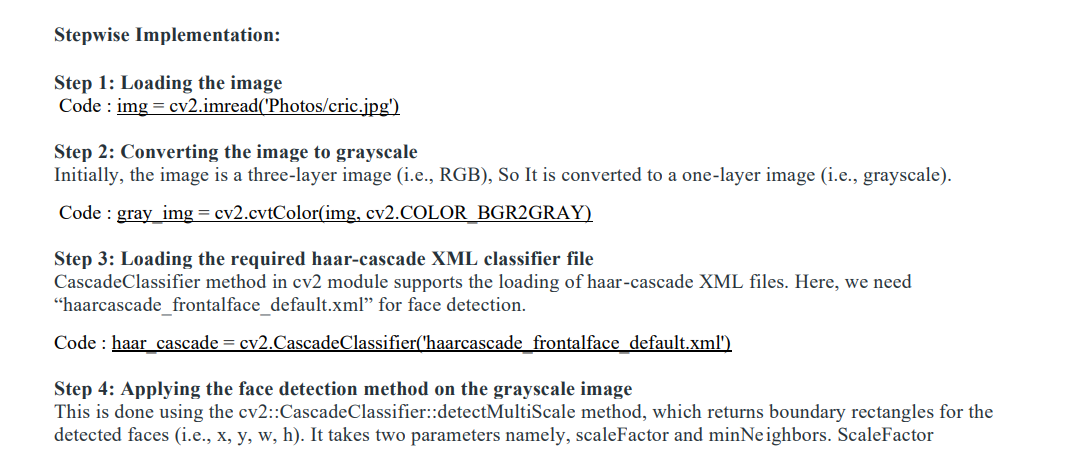
\includegraphics[width=1.3\textwidth]{step.png}
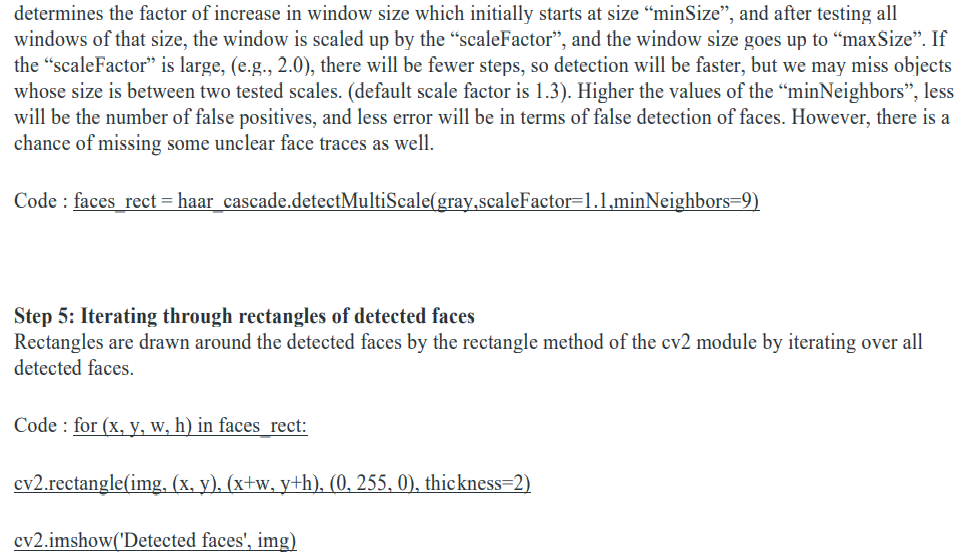
\includegraphics[width=1.3\textwidth]{step2.png}



\section {Below is the implementation :}


\includegraphics [width=0.9\textwidth]{pic.png}\\
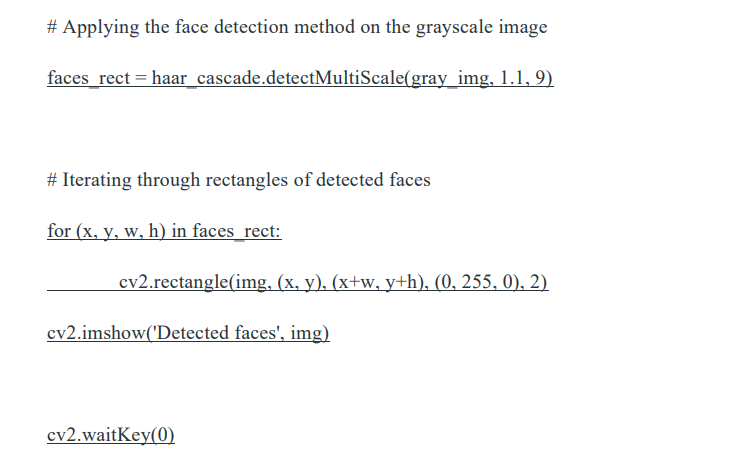
\includegraphics[width=0.9\textwidth]{pro.png}
\newpage
\section {CONCLUSION}
The aim is to automate and make a system that is useful to the organization such as an institute. The efficient and accurate
method of attendance in the office environment that can replace the old manual methods. This method is secure enough,
reliable and available for use.
No need for specialized hardware for installing the system in the office. It can be constructed using a camera and
computer. Human face detection can be used in different fields, such as in law enforcement, equity arrangements,
identification recovery, and Biometrics.
Facial identity and recognition technology integrate university campus tech solutions to ensure student protection. For
chosen locations, such as university campuses, we establish facial recognition based on face detection.
Our primary point is to identify and throw unwanted persons out of the protected area. We are eager to develop a quick
and efficient framework of facial recognition that identifies and does not reach people's faces.
By calculating the illegal movement of outsiders by using our suggested methodology, we will minimize internal campus
crimes much as our point is to expand transparent mindfulness, human protection, and authorization of the law by
adopting our proposal. In the future we will add artificial intelligence over the proposed system, to differentiate
objects like humans, animals, and so on to ensure security surveillans

\section {REFERENCES}
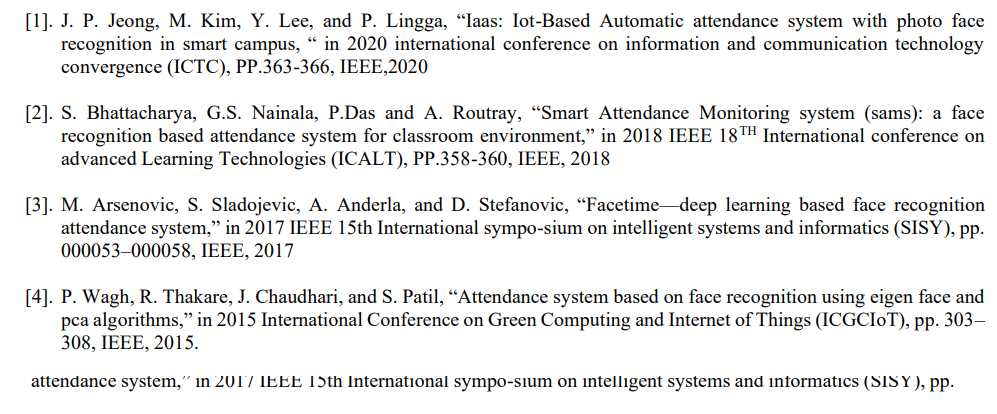
\includegraphics[width=0.9\textwidth]{ref.png}\\
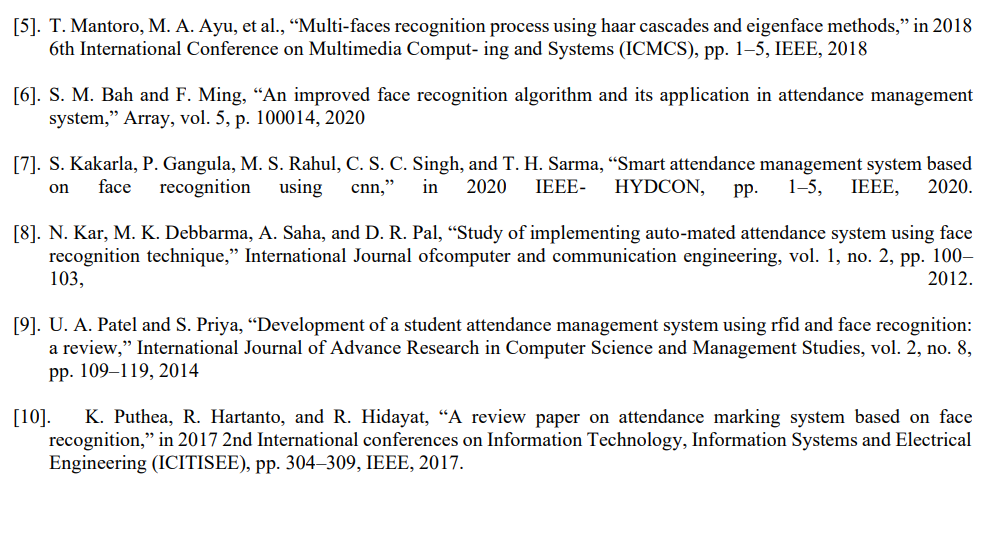
\includegraphics[width=0.9\textwidth]{ref2.png}



